
%\documentclass[letterpaper, 10 pt, conference]{ieeeconf}
\documentclass[letterpaper, 10 pt,  conference, twoside]{IEEEtran/IEEEtran}

\IEEEoverridecommandlockouts

%\overrideIEEEmargins

% The following packages can be found on http:\\www.ctan.org
\usepackage{graphics} % for pdf, bitmapped graphics files
\usepackage{graphicx}
\usepackage{epsfig} % for postscript graphics files
%\usepackage{mathptmx} % assumes new font selection scheme installed
%\usepackage{times} % assumes new font selection scheme installed
\usepackage{amsmath} % assumes amsmath package installed
\usepackage{amssymb}  % assumes amsmath package installed
\usepackage{amsthm,array}
\usepackage{algorithm}
\usepackage[noend]{algpseudocode}
\usepackage[noadjust]{cite}
\usepackage{balance}
%\usepackage[utf8]{inputenc}
\usepackage[english]{babel}

\theoremstyle{definition}
\newtheorem{definition}{Definition}[section]
\newtheorem{prop}{Proposition}
\newtheorem{theorem}{Theorem}
\begin{document}
\title{A Decentralized Ergodic Control Approach to the Multi-Agent Pursuit-Evasion Problem}

\author{Ian Abraham and Todd D. Murphey
\thanks{Authors are with the Neuroscience and Robotics Laboratory (NxR) at the Department of Mechanical Engineering$^{1}$, Northwestern University, 2145 Sheridan Road Evanston, IL 60208 USA.}
\thanks{{\tt\small Email: i-abr@u.northwestern.edu, t-murphey@northwestern.edu}}
}
\maketitle

\begin{abstract}
In this work, we present ergodic control as a method for solving the pursuit-evasion problem for nonlinear continuous systems.
We show that adopting an ergodic control policy the pursuit-evasion problem obtains a Nash equilibrium.
Ergodic control is then formulated for a decentralized network of robotic agents. It is shown that the decentralized ergodic control problem is equivalent to solving the centralized ergodic control problem when the network of agents has reached consensus over the past exploration of each agent. Examples are presented for the application of ergodic theory for exploring information-based distributions, localization of multiple targets, and estimation of spatial terrain. Each example emphasizes the ease with which ergodic control can be decentralized and the benefits of a decentralized network of agents actively exploring.
\end{abstract}

\section{Introduction}

Within the field of autonomous mobile robots, active exploration has been a fundamental area of research. Specifically, exploration and mapping of unknown environments has led to the development of various SLAM-like algorithms \cite{bailey2006simultaneous, durrant2006simultaneous, choset2001topological}. Recent work in active exploration has utilized the concept of optimally sensing based on the particular sensory modalities available to the robot \cite{abraham2017ergodic, de2016ergodic, miller2016ergodic, yang2013human, ts_ref_1}. This desire to encode exploratory behavior in robotics has largely been inspired by biology \cite{iida2016biologically, zhu2015bioinspired}. In particular, the need for unique exploratory behavior subject to constraints imposed by sensory modalities like visual and tactile has led to advances in the use of information theory for active exploration \cite{abraham2017ergodic, miller2016ergodic, mihaylova2002comparison, ryan2010particle}. A clear extension to much of the previously mentioned work is application in multi-agent robotic networks.

Within the field of active exploration distributed robot networks have been shown to improve the efficiency and span of exploration of mobile robots \cite{carmel1999exploration, dudek1996taxonomy, manss2016decentralized}. Moreover, the application of distributed robotic networks take into consideration the specifications of the task and effectively use the underlying network connection for improved performance \cite{manss2016decentralized, viseras2014efficient, khamis2014adaptive, pei2014distributed}. Interestingly, many of the underlying centralized version of the active exploration methods are shown to be preserved with the use of network consensus. Existing work in applications of ergodic theory in active exploration (or ergodic exploration for short) has been formulated in a centralized multi-agent system for linear dynamics \cite{mathew2011metrics}. In addition, work has been done on synthesizing controllers for multi-robot systems using ergodic processes \cite{shell2006ergodic}. However, it has yet to be shown how such a network would benefit from network consensus or whether it can be extended to nonlinear dynamical systems.

In this work, we contribute a formulation of an ergodic controller for active exploration. Specifically, we formulate the controller for nonlinear dynamical systems using sequential action control \cite{ansari2016sequential}. The formulation is then extended to a centralized connected robotic network. We then formulate a decentralized ergodic controller and show that under consensus, the objective of the decentralized ergodic controller is equivalent to the objective of the centralized ergodic controller. Numerical examples are presented that show the versatility in ergodic control when applied to exploration, localization, and mapping problems. In particular, these examples emphasize the ease with which ergodic control can be extended to variations of problems within distributed mobile robotics.

The paper is outlined as: Section \ref{sec:ergcontrol} formulates the ergodic optimal control problem and then presents ergodic control in a centralized and decentralized manner. Section \ref{sec:network} discusses the network chosen in this work and its effect on ergodic control. Section \ref{sec:est} extends the ergodic control formulation for problems in exploration, estimation and localization. Last, sections\ref{sec:res} and \ref{sec:conc} present simulation results and conclusion of the application of a connected decentralized ergodic controller.

\section{Ergodic Control} \label{sec:ergcontrol}

In this section, we define the variants of the ergodic control problem. We first start with a formulation of ergodic control for a nonlinear system through a similar process as done with sequential action control~\cite{ansari2016sequential}. Following the derivation of ergodic control, we modify the specification of the ergodic controller for control of a centralized multi-agent system. We then show in the next section a derivation of a decentralized ergodic controller for a single agent in the multi-agent system and show that under consensus of the network the optimal control solution to the decentralized problem is equivalent to the optimal control solution of the centralized ergodic control problem.

\subsection{Canonical Ergodic Control}
The ergodic exploration problem is defined for a control-affine dynamical systems of the form
\begin{equation} \label{eq:caff}
\dot{x} = f(x,u) = g(x) + h(x) u .
\end{equation}
Ergodic control is formulated as the control solution that minimizes the ergodic metric
\begin{equation}
\mathcal{E}(x(t)) = \sum_{k \in \mathbb{Z}}(\phi_k - c_k)^2
\end{equation}
where
\begin{equation}
\phi_k = \int_X \Phi(x) F_k (x) d x
\end{equation}
and
\begin{equation}
c_k = \frac{1}{T}\int_{t_0}^{t_0 +T} F_k(x(t)) dt
\end{equation} for some time $t_0$ to $t_0+T$.
Here, $\Phi(x)$ is the underlying spatial distribution (we will sometimes refer to this as the target distribution since it is being used as a reference for the control system) and $F_k(x)$ is the basis function\footnote{In this work, the cosine basis function is used, however, any choice of basis function $F_k$ can be used.}. Agent actions $x(t)$ are considered to be ``ergodic'' with respect to a target distribution $\Phi(x)$ when the time averaged statistics of the robots actions are equivalent to the statistics of the target distribution.

We define the objective of the ergodic control problem as
\begin{equation*}
\begin{aligned}
& \underset{u}{\text{minimize}}
& & \mathcal{E}(x(t)) \\
& \text{subject to}
& & \dot{x}(t) = f(x(t), u(t)) .
\end{aligned}
\end{equation*}
Instead of minimizing directly over control $u$, we consider the first order sensitivity to control application time $\lambda$. This is found by taking the derivative of $\mathcal{E}$ with respect to infinitesimal control application time $\lambda$ defining the mode insertion gradient as
\begin{equation} \label{eq:mode_insert}
\begin{aligned}
& & \frac{d \mathcal{E}}{d\lambda} &= \rho (s) ^T (f_2(s,s) - f_1(s)) \\
\text{subject to}
& & \dot{\bold{\rho}} &= - \sum_{k \in \mathcal{Z}}(\phi_k - c_k) \frac{\partial F_k(x)}{\partial x} - \frac{\partial f}{\partial x }^T \rho .
\end{aligned}
\end{equation}
In the definition of $ \frac{d \mathcal{E}}{d\lambda}$
\begin{equation*}
f_1(t) = f(x(t), u_1 (t))
\end{equation*}
and
\begin{equation*}
f_2(t, \tau) = f(x(t), u_2 (\tau))
\end{equation*}
are the systems' state $f$ subject to the default control $u_1$ and optimal control $u_2$. Following the formulation of sequential action control (SAC) \cite{ansari2016sequential} we define an auxiliary objective function $J_2$ as
\begin{equation*}
J_2 = \frac{d \mathcal{E}}{d \lambda} + \frac{1}{2}\Vert u_2 - u_1 \Vert_R^2
\end{equation*}
whose minimum occurs when the mode insertion gradient is most negative, regularized by the change in the default control $u_1$ with $R$ as a diagonal positive definite matrix. Since $J_2$ is convex in $u_2$, taking a first-order optimality approach to solve for an optimal $u_2$ gives the closed form solution
\begin{equation}
u^*(t) = -R^{-1}h(x)^T\rho(t) + u_1(t).
\end{equation} The time of control application $\lambda$ that significantly reduces the ergodic cost is obtained via
\begin{equation}
\lambda ^*= \underset{\lambda}{\text{argmin }} \frac{d\mathcal{E} (\lambda)}{d\lambda} ,
\end{equation}
typically approximated using a line search.
Thus, at each sampling instance $t_{curr}$, the ergodic controller forward predicts the system trajectory based on the sequence of control actions $u_1$. The sensitivity to that trajectory is calculated via the mode insertion gradient (\ref{eq:mode_insert}) and then  used to create the closed form solution of control actions that reduce the ergodic metric. The time of application that significantly reduces the ergodic cost is then calculated and the controller returns $u^*(\lambda)$ which is added to the schedule of control actions $u_1$.
\subsection{Centralized Ergodic Control}
In a similar formulation as the canonical ergodic control problem, we define the centralized ergodic control problem for a network of robot agents $x_i(t)$ subject to dynamical constraints of the form
\begin{equation*}
\dot{x}_i(t) = f_i(x_i , u_i) = g_i(x_i) + h_i(x_i)u_i .
\end{equation*}
We can define the ergodic metric as before in a centralized manner as
\begin{equation}\label{eq:cerg}
\mathcal{E} (x (t)) = \sum_{k \in \mathbb{Z}} (\phi_k - c_k (x (t))^2
\end{equation}
where
\begin{equation*}
x =
\begin{bmatrix}
x_i \\
\vdots \\
x_N
\end{bmatrix}
\end{equation*}
is the stacked centralized representation of all robot agent $x_i (t) \forall i \in \{1, \ldots, N \}$. For a network of $N$ agents, the time averaged spatial statistical representation of the collective robot network, $c_k$, is defined as
\begin{equation} \label{eq:ckn}
c_k = \frac{1}{T} \int_{t_0}^{t_0 + T} \frac{1}{N} \sum_i^N F_k(x_i(t)) = \frac{1}{T} \int_{t_0}^{t_0+T} \tilde{F}_k(x(t))
\end{equation}
where $\tilde{F}_k(x(t)) = \frac{1}{N} \sum_j^N F_k(x_i(t))$. Here, the mode insertion gradient is given as
\begin{equation*}
\frac{d \mathcal{E}}{d\lambda} = \rho(s)^T (f(x(s), u_2(s)) - f(x(s),u_1(s)))
\end{equation*}
where
\begin{equation*}
\bold{\rho}(t) =
\begin{bmatrix}
\rho_i \\
\vdots \\
\rho_N
\end{bmatrix} ,
f =
\begin{bmatrix}
f_i \\
\vdots \\
f_N
\end{bmatrix} .
\end{equation*}
The solution to the costate equation $\rho$ is obtained via the backwards differential equation
\begin{equation*}
\dot{\bold{\rho}} = - q\sum_{k \in \mathcal{Z}}(\phi_k - c_k) \frac{\partial \tilde{F}_k(x)}{\partial x} - \frac{\partial f}{\partial x }^T \rho
\end{equation*}
which is the exactly the same as (\ref{eq:mode_insert}).
Assuming that each robot's state $x_i(t)$ is independent of one another, we see that
\begin{equation*}
\frac{\partial \tilde{F}_k(x)}{\partial x} =
\begin{bmatrix}
\frac{\partial F_k(x_i)}{\partial x_i} \\
\vdots \\
\frac{\partial F_k(x_N)}{\partial x_N}
\end{bmatrix}
\end{equation*}
and
\begin{equation*}
\frac{\partial f}{\partial x} =
\begin{bmatrix}
\frac{\partial f_i}{\partial x_i} & 0 & \ldots & 0 \\
0 & \frac{\partial f_{i+1}}{\partial x_{i+1}} \\
\vdots & & \ddots  & \\
0 &  & & \frac{\partial f_N}{\partial x_N}
\end{bmatrix}.
\end{equation*}
As done previously, we define a secondary cost function
\begin{equation}  \label{eq:aux2}
J_2 = \frac{d \mathcal{E}}{d \lambda} + \frac{1}{2}\Vert u_2 - u_1 \Vert_R^2.
\end{equation}
where $R$ is a positive-definite diagonal matrix with elements $R_i$.
Taking the derivative of (\ref{eq:aux2}) with respect to control $u_2$ and setting the resulting expression equal to zero gives
\begin{equation} \label{eq:opt_contr}
u^* (t) = -R^{-1} h(x)^T \rho(t) + u_1(t).
\end{equation}
If we expand (\ref{eq:opt_contr}) we get
\begin{equation*}
\resizebox{0.45 \textwidth}{!}
{ $
\begin{bmatrix}
u^*_i (t) \\
\vdots \\
u^*_N(t) \\
\end{bmatrix}
=
-R^{-1}  \begin{bmatrix}
h_i(x_i) & \\
& \ddots & \\
& & h_N(x_i)
\end{bmatrix}^T
\begin{bmatrix}
\rho_i (t) \\
\vdots \\
\rho_N(t)
\end{bmatrix}
 +
 \begin{bmatrix}
 u_{1,i} (t) \\
 \vdots \\
 u_{1,N}(t)
 \end{bmatrix}
. $
}
\end{equation*}
Since $h(x)$ is a block diagonal matrix, the transpose of a block diagonal matrix is the transpose of each element on the diagonal. With $R$ as a positive definite diagonal matrix whose diagonal elements $R_i$ are unique to each agent, we find the solution that minimizes (\ref{eq:aux2}) with respect to the control $u_2$ is
\begin{equation} \label{eq:central}
\begin{bmatrix}
u^*_i (t) \\
\vdots \\
u^*_N(t)
\end{bmatrix}
=
\begin{bmatrix}
-R_i^{-1} h_i(x_i)^T \rho_i(t) + u_{1,i}(t) \\
\vdots \\
-R_N^{-1} h_N(x_N)^T \rho_N(t) + u_{1,N}(t) \\
\end{bmatrix}
\end{equation}
which is the stacked representation of the control solution that reduces the ergodic metric for each individual agent. As done before, finding the time of control application that significantly reduces the ergodic metric for all agents is found via
\begin{equation*}
\lambda ^*= \underset{\lambda}{\text{argmin }} \frac{d\mathcal{E} (\lambda)}{d\lambda} .
\end{equation*}
The rest of the controller follows the same formulation as the canonical ergodic control problem.
\subsection{Decentralized Ergodic Control}

The derivation of the decentralized ergodic control problem first assumes that there exists an underlying connected network for which each agent can communicate with one another. Assume that the connections can be represented via a graph Laplacian $L$ \cite{deo2016graph}. A consensus matrix $P$ can be generated from the graph Laplacian such that $P$ is both row and column stochastic \cite{deo2016graph, bertsekas1989parallel}. In the decentralized case, the ergodic metric is defined as
%\begin{equation}
%\mathcal{E}_i(x_i(t)) = \sum_{k \in \mathbb{Z}} (\phi_k - \sum_j (P \otimes I_{\vert k \vert})_{ij} c_{k,j})^2
% \end{equation}
 \begin{equation} \label{eq:derg}
\mathcal{E}_i(x_i(t)) = \sum_{k \in \mathbb{Z}} (\phi_k - \sum_j P_{ij} c_{k,j})^2
 \end{equation}
for each agent $i$ with neighbors $j$. The consensus matrix $P$ is used to transmit information about where each agent has explored (and is going to explore) to neighboring agent. As a result of sharing this information, each agent is able to synthesize a control solution that is sensitive to what the network of agents has explored. Hence, consensus improves exploration efficiency for the overall network.

Following the derivation of the centralized ergodic controller, the mode insertion gradient for an individual agent is then,
\begin{equation*}
\frac{d \mathcal{E}_i}{d \lambda} = \rho_i(s) (f_i(x_i(s), u_{2,i}(s)) - f_i(x_i(s), u_{1,i}(s)))
\end{equation*}
with the costate equation obtained from the backwards-differential equation
%\begin{equation}
%\dot{\rho}_i = - \sum_{k \in \mathcal{Z}}(\phi_k - \sum_j (P \otimes I_{\vert k \vert})_{ij} c_{k,j}) \frac{\partial F_{k,i}(x_i)}{\partial x_i} - \frac{\partial f_i}{\partial x_i }^T \rho_i.
%\end{equation}
\begin{equation*}
\dot{\rho}_i = - \sum_{k \in \mathcal{Z}}(\phi_k - \sum_j P _{ij} c_{k,j}) \frac{\partial F_{k,i}(x_i)}{\partial x_i} - \frac{\partial f_i}{\partial x_i }^T \rho_i.
\end{equation*}
The solution to the secondary cost function for an individual agent
\begin{equation*}
J_{2,i} = \frac{d \mathcal{E}_i}{d \lambda} + \frac{1}{2} \Vert u_{2,i} - u_{1,i}\Vert ^2_{R_i}
\end{equation*}
is
\begin{equation}
u^*_i(t) = -R_i^{-1} h_i(x_i)^T \rho_i(t) + u_{1,i}(t)
\end{equation}
which is equivalent to the individual agent's control solution as the stacked representation of the centralized case (\ref{eq:central}). Individual time of control application $\lambda$ can be found with
\begin{equation*}
\lambda ^*= \underset{\lambda}{\text{argmin }} \frac{d\mathcal{E}_i (\lambda)}{d\lambda} .
\end{equation*}
%However, the time of action of one agent may interfere with another agent, impeding on reduction of the ergodic metric. This can be solved by having a consensus on the first order sensitivity of control application and finding the time of application that achieves the largest decrease in the ergodic metric. This can be written as
%\begin{equation}
%\lambda ^*= \underset{\lambda}{\text{argmin }} N\sum_j P_{ij} \frac{d \mathcal{E}_j (\lambda)}{d\lambda}
%\end{equation}
%and is equivalent to finding the time of control application in the centralized ergodic control formulation.

\begin{theorem}
For a connected network of agents with control-affine dynamics (\ref{eq:caff}), the decentralized ergodic control problem (\ref{eq:derg}) is equivalent to the centralized ergodic control problem (\ref{eq:cerg}) when a consensus on the $c_{k,i}$ values is reached.
\end{theorem}
{\it Proof: } Assume there exists a consensus matrix $P$ that is row and column stochastic and described a connected graph. The operation $ \sum_j P_{ij} c_{k,j}$ is equivalent to taking an average of the local $c_k$ values for each neighboring agent $j$. Thus, we can rewrite the consensus on $c_k$ as
%\begin{equation}
%\sum_j (P \otimes I_{\vert k \vert})_{ij} c_{k,j} = \frac{1}{N}\sum_j \frac{1}{T} \int_{t_0}^{t_0 +T} F_k(x_j(t)) dt.
%\end{equation}
\begin{equation}
\lim_{t_k \to \infty}\sum_j P_{ij}^{t_k} c_{k,j} = \frac{1}{N}\sum_j \frac{1}{T} \int_{t_0}^{t_0 +T} F_k(x_j(t)) dt.
\end{equation}
where $t_k$ is the number of times that the $P_{i,j} c_{k,j}$ values have been iterated upon. The summation over all neighboring agents can be brought into the integral to give
%\begin{equation}
%\begin{aligned}
% \sum_j (P \otimes I_{\vert k \vert})_{ij} c_{k,j} &=  \frac{1}{T} \int_{t_0}^{t_0 +T} \frac{1}{N}\sum_j F_k(x_j(t)) dt \\
%&= \frac{1}{T} \int_{t_0}^{t_0 +T} \tilde{F}_k(x(t)) dt
%\end{aligned}
%\end{equation}
\begin{equation}
\begin{aligned}
\lim_{t_k \to \infty}\sum_j P_{ij}^{t_k} c_{k,j} &=  \frac{1}{T} \int_{t_0}^{t_0 +T} \frac{1}{N}\sum_j F_k(x_j(t)) dt \\
&= \frac{1}{T} \int_{t_0}^{t_0 +T} \tilde{F}_k(x(t)) dt
\end{aligned}
\end{equation}
which when $t_k \to \infty$, a consensus is reached on where each agent has explored. Thus for any connected graph, the consensus is equivalent to (\ref{eq:ckn}).

Regardless of whether consensus amongst agents is reached, the ergodic measure for an individual agent will still be reduced asymptotically as $t \to \infty$. Consider that there exists a control action $u$ that minimizes the ergodic cost (\ref{eq:derg}). Then the mode insertion gradient (\ref{eq:mode_insert}) is $\le 0$ for some $u^*(\lambda)$ which defines the rate of reduction of the cost at time $\lambda$. As a result, any partial consensus will be included in the sensitivity of the ergodic metric with respect to neighboring agents' actions. Thus, consensus only impacts the rate of convergence of the ergodic metric and is dependent on the network connectivity.

\section{Network and Consensus} \label{sec:network}

In the previous section, we described the effects of consensus on the decentralized ergodic controller. In particular, the rate of convergence for both minimization of the ergodic metric and consensus on the $c_k$ values of each agent depend on the connectivity of the graph itself. In this section, we discuss the formulation of the consensus matrix $P$ that can be used for the decentralized ergodic controller.

\begin{figure}[th]
\centering
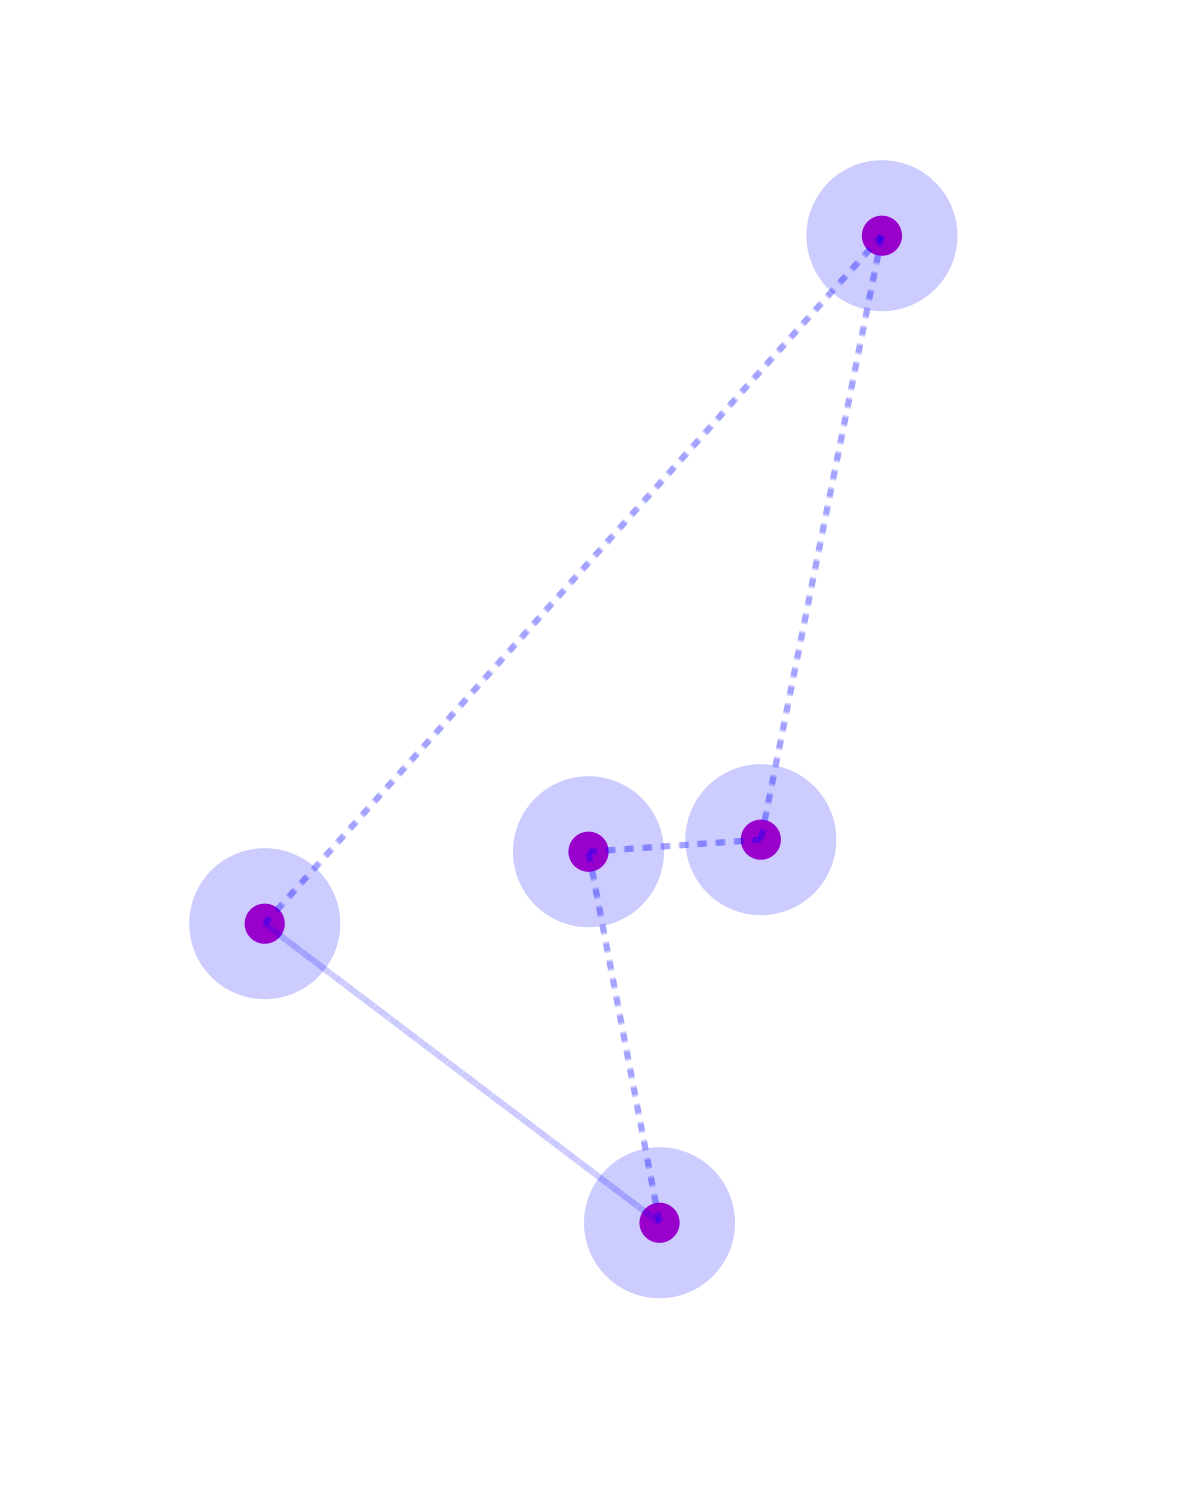
\includegraphics[scale=0.4]{figures/5networkpath.png}
\caption{ A ring network connection defined for a set of $n$ vertices with edges $(i,i+1) \cup (n,1)$ for $i \in \{1, \ldots, n\}$ is used for localization and estimation examples. The dotted lines represent the connection between each agent. Each agent is represented by the circle. }
\label{fig:path}
\end{figure}

For the decentralized ergodic controller, any consensus matrix can be designed so long as the consensus matrix is row and column stochastic. This implies that the resulting consensus matrix must approximate the average of all the agents' $c_k$ values. In an ideal situation where the graph is fully connected, consensus of the $c_k$ values will occur rapidly. However, as shown in the last section, even partial consensus will improve the rate of convergence of the ergodic metric. In a later discussion in the results, convergence of the ergodic measure is presented with a 1, 2, and 3 agent network with a complete graph topology. For the remainder of this work, a ring graph (see Fig.~\ref{fig:path}) is used as an arbitrary choice to show that the decentralized ergodic controller eventually reaches a consensus so long as the graph is connected. Future work will involve examining various consensus matrices and their effects on the rate of convergence of the ergodic metric.

\section{Estimation and Localization} \label{sec:est}

In this section we present a formulation of the decentralized ergodic control for estimation and localization problems. In general, problems of exploration for distributed information will take the same form as was developed initially in section~\ref{sec:network} where the spatial statistical distribution $\Phi$ is given.

\subsection{Estimation}

Typically estimation problems are formulated as a minimization of the sum of square errors of a set of measurement data $y_i$ taken at state $x_i \in \mathbb{R}^n$ and a prediction of the underlying measurement model that is likely to represent the data $\phi(\theta, x)$ where $\theta$ is some parameter that is to be estimated. Formally, the least-squares problem is described as
\begin{equation} \label{eq:leastSquares}
\begin{aligned}
& \underset{\theta}{\text{min}} \sum_{i}^{N} (y_i - \phi(\theta, x))^2
\end{aligned}
\end{equation}
Solutions to this problem exist in abundance \cite{marquardt1963algorithm, julier1997new, wan2000unscented}. There exists an equal abundance of work in estimation for distributed networks \cite{carli2008distributed, liu2014distributed, arablouei2014distributed}. In this work, we utilize a distributed Kalman filter \cite{carli2008distributed}, however any estimator which provides a statistical representation $p(\theta)$ over the set of parameters $\theta$ is sufficient for use in ergodic control. The only significant change in the ergodic control formulation is the target distribution $\Phi(x)$.

For an estimation problem, we utilize the expected information density (EID) of the estimator. The EID is first formulated with the definition of the Fisher information matrix given as
\begin{equation}
I(\theta, x) = \frac{\partial \phi(\theta, x)}{ \partial \theta} ^T \Sigma^{-1} \frac{\partial \phi(\theta, x)}{ \partial \theta}
\end{equation}
where $\Sigma^{-1}$ is the measurement covariance. The EID is then the expectation of information given the certainty of the estimated parameters, $p(\theta)$. That is, we define the EID as
\begin{equation}
\text{EID}(x) = \eta \int_\theta I(\theta, x) p(\theta) d\theta
\end{equation}
where $\eta$ is a normalization factor. For multi-parameter estimation, the determinant of the EID is defined as our target distribution $\Phi(x)$ which implies that each individual agent in the distributed network will have their own $\phi_k$ values given by
\begin{equation}
\phi_{k,i} = \int_X \text{det}\vert \text{EID}_i(x)\vert F_k(x) dx.
\end{equation}
However, consensus on each $\phi_{k,i}$ is not necessary as we are using estimators that form a consensus on the parameters $\theta$ and their statistical parameters \cite{carli2008distributed}. Thus, the only modification to the distributed ergodic control formulation is the need to recalculate $\phi_k$ whenever a new estimate of $\theta$ is provided. In this work, we use the example of mapping the terrain of a square domain region. Thus, measurements are considered to be local topological height.

\subsection{Target Localization}

Target localization is treated in the same manner as an estimation problem. Specifically, we are estimating the location of targets in the environment. In this work, we examine target localization in an environment filled with obstacles. A benefit of the formulation of ergodic control is the ease with which the objective function can be formulated. We assume that each robot has a map of the environment $\Gamma(x)$ that penalizes the robot if it is in collision with the obstacle. The primary objective function for each agent then becomes
\begin{equation}
\mathcal{E}_i(x_i(t)) = q_1\sum_{k \in \mathbb{Z}} (\phi_k - \sum_j P_{ij} c_{k,j})^2 + q_2\Gamma(x)
 \end{equation}
where the mode insertion gradient is
\begin{equation*}
\frac{d \mathcal{E}_i}{d \lambda} = \rho_i(s) (f_i(x_i(s), u_{2,i}(s)) - f_i(x_i(s), u_{1,i}(s)))
\end{equation*}
with the costate solved by the backwards differential equation
\begin{equation*}
\resizebox{0.5 \textwidth}{!}
{ $
\dot{\rho}_i = - 2 q_1\sum_{k \in \mathcal{Z}}(\phi_k - \sum_j P _{ij} c_{k,j}) \frac{\partial F_{k,i}(x_i)}{\partial x_i} - q_2\frac{\partial \Gamma(x_i)}{\partial x_i}- \frac{\partial f_i}{\partial x_i }^T \rho_i .
$
}
\end{equation*}
Thus, during forward trajectory prediction, the sensitivity will include future collisions that may occur.

Here, measurements $y_i$ are taken as global position measurements of the target relative to the world frame. Each robot will then have a sensor with a limited circular range $r$. Initially, none of the agents know the location of any of the targets, thus the EID is considered to be a uniform distribution.

The results for exploration, estimation, and target localization are shown in the following section.

\section{Results} \label{sec:res}

In this section, results are presented for three applications of decentralized ergodic control. The first example discusses the reduction of the ergodic measure during information-based exploration of a unknown distribution. In particular, we observe the effects of introducing agents in a complete graph network configuration (defined as a graph with $n$ vertices connected to all other vertices) and collaborative behavior amongst agents. The second example illustrates the improvement in area coverage for localizing targets in a crowded environment. The last example illustrates how the decentralized ergodic controller can be used for Fisher Information-based estimation of terrain topology.

\subsection{Information-Based Coverage}

Information-based exploration is presented with an example comparing coverage of a distribution using a 1, 2, and 3 agent network. The task for each agent is to maintain coverage of a distribution (see Fig.~\ref{fig:n_agent}) that is proportional to the information available (given by the heat map). This example is presented to illustrate the collaborative behavior of decentralized ergodic control when under consensus. Specifically, this collaborative behavior can be seen in the trajectory traces of the 2 and 3 agent network. Each agent covers one of the peaks of the distribution while the other spans the remaining peaks. The agents then trade off this behavior to get an improved reduction of the ergodic measure. The benefit of using a multi-agent distributed ergodic system is shown in the ergodicity measure in Fig.~\ref{fig:n_agent} where the rate of reduction in the ergodic metric increases with added agents.

\begin{figure}[ht!]
\centering
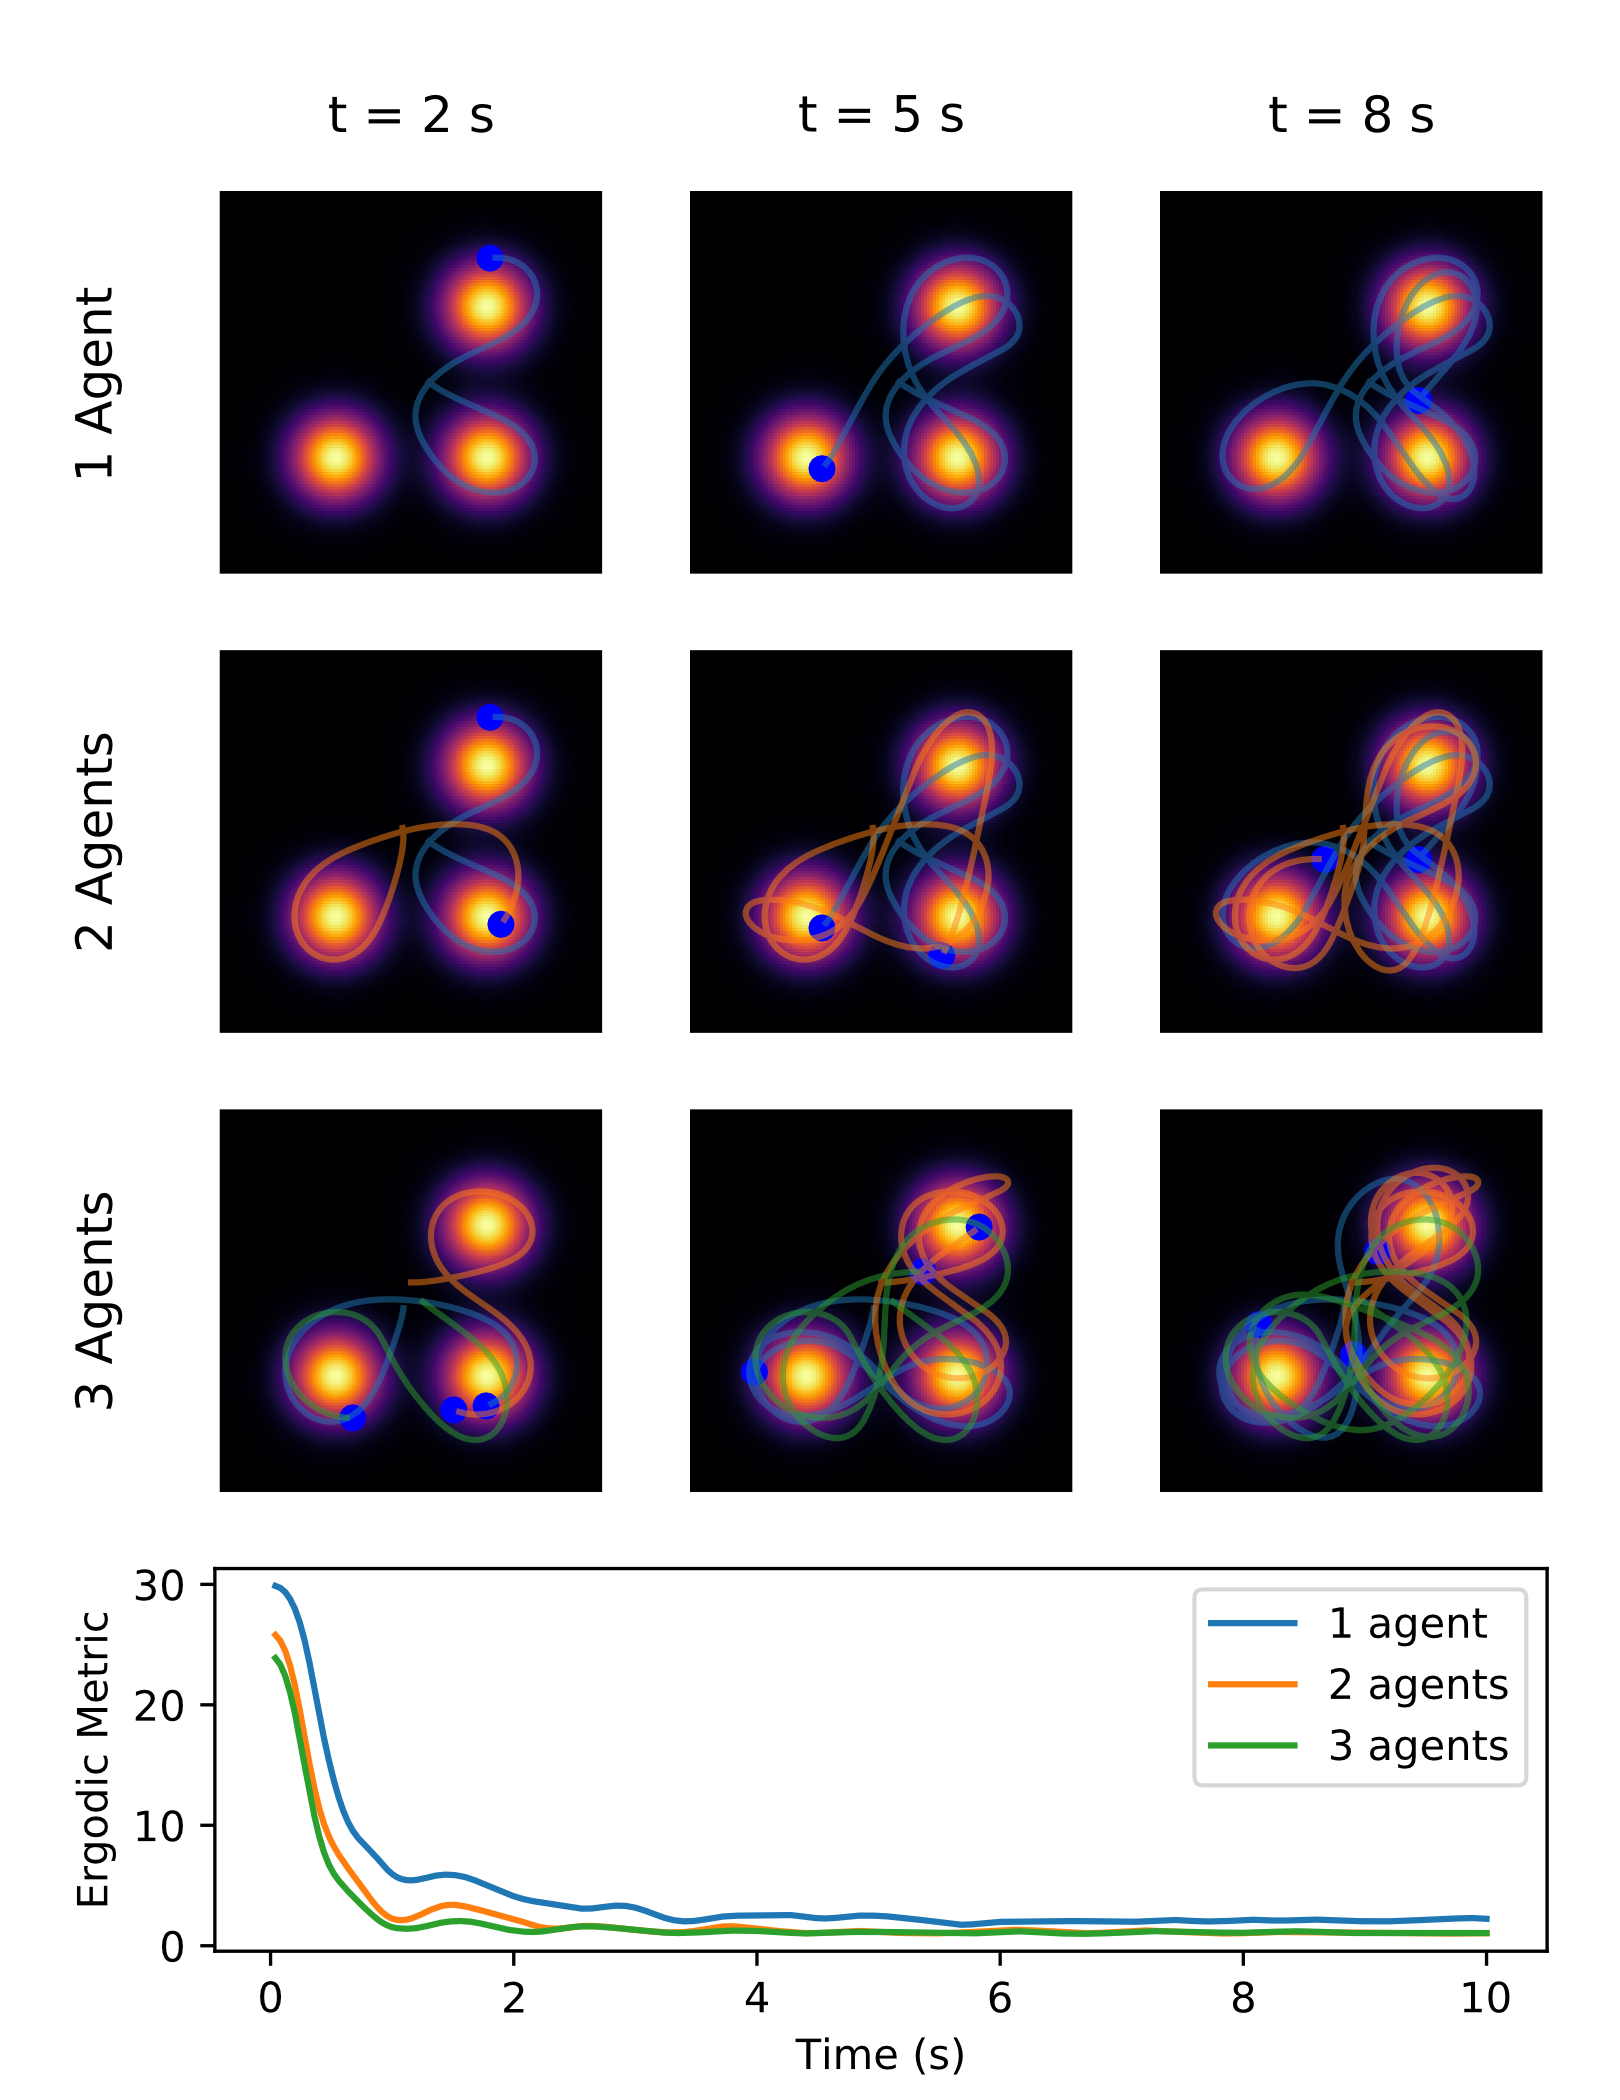
\includegraphics[scale=0.6]{figures/n_agent_comparison2.png}
\caption{ Information based exploration is shown with 1, 2, and 3 agents using ergodic control. Adding an additional agent automatically improves the coverage and reduction of the ergodic metric. Collaborative behavior is seen with the 2 and 3 agent systems where a trade-off occurs allowing a single agent to spend more time at a peak while the other agents span across the remaining information peaks. }
\label{fig:n_agent}
\end{figure}

\begin{figure*}[th!]
\centering
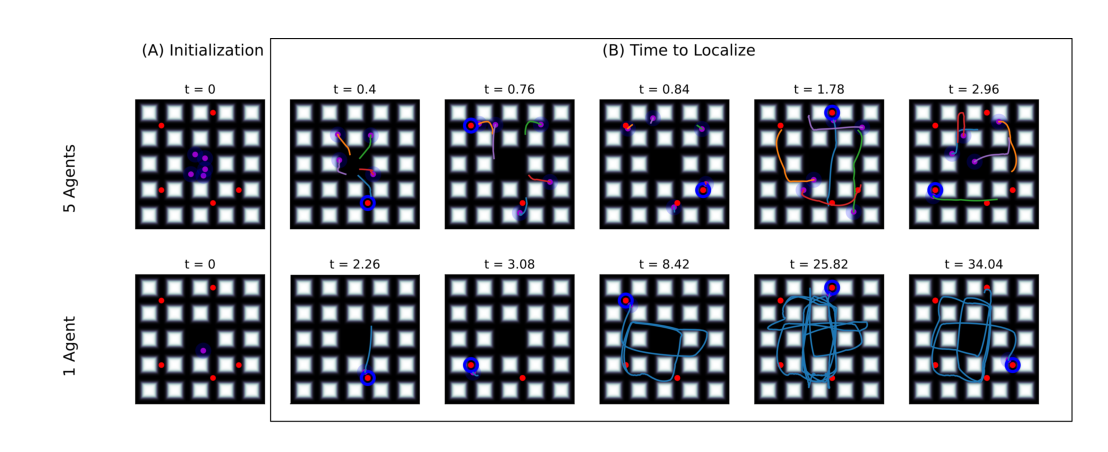
\includegraphics[scale=0.9]{figures/distr_loc2.eps}
\caption{ Localization of 5 targets in an environment with obstacles is shown for a single agent and a 5 agent network shown in Fig.~\ref{fig:path}. Each time frame shown indicates when a new agent was discovered in the environment. (A) The starting frame $t=0$ shows the starting location of each agent. Note that the 5 agent network distributes exploration amongst the agents which results in finding all 5 targets within $3$ seconds. Interestingly, ergodic exploration of 1 agent eventually results in the localization of all 5 agents given enough time to explore the environment. A monte-carlo simulation of the network localizing sequentially randomly generated targets is provided in the link: https://vimeo.com/209261679/0d65c1a9ac .}
\label{fig:disloc}
\end{figure*}

\subsection{Localization}

Results for localization are presented with the task to localize 5 targets within an environment with obstacles (see Fig.~\ref{fig:disloc}). Targets are shown as a red dot and initialized in the same way for a network of 1 agent and 5 agents. Each time an agent is localized, a blue circle is drawn at the time of localization from the initial starting point (Fig.~\ref{fig:disloc}). Each agent is not allowed to traverse the grey obstacles in the environment. Results show a clear benefit of utilizing consensus within ergodic exploration. Specifically, each individual agent explores their own particular subset of the environment. Therefore, each individual agent travels less which improves the overall energetic cost of moving while localizing all the targets at a much faster rate than with a single agent. The longer travel times are clearly noted in the trajectory traces of the single robot agent localizing the targets. Although the single agent requires longer time to localize all the targets, the ergodic control still successfully synthesizes actions that enable a single agent to span a large enough region to eventually localize all the targets.

The analysis of the localization example is furthered with a detailed observation of the ergodic measure. Figure~\ref{fig:disloc_conv} shows the convergence of the ergodic metric for the single agent, the collective 5 agent network, and the individual measures of ergodicity for each agent in the 5 agent network. With more agents, the ergodic measure reduces rapidly and is maintained in a non zero equilibrium value (this is due to the measure never being able to reach zero). The individual robotic agents ergodicity measures show similarity with the single agent network. Thus, regardless if consensus is reached, each agent will reduce the ergodic measure at their own particular rate. As consensus is reached, the rate of decent of the ergodic metric increases. When information about where each agent has explored is transferred through the network, the individual efforts result in an overall reduction in the ergodic metric.

\begin{figure}[!h]
\centering
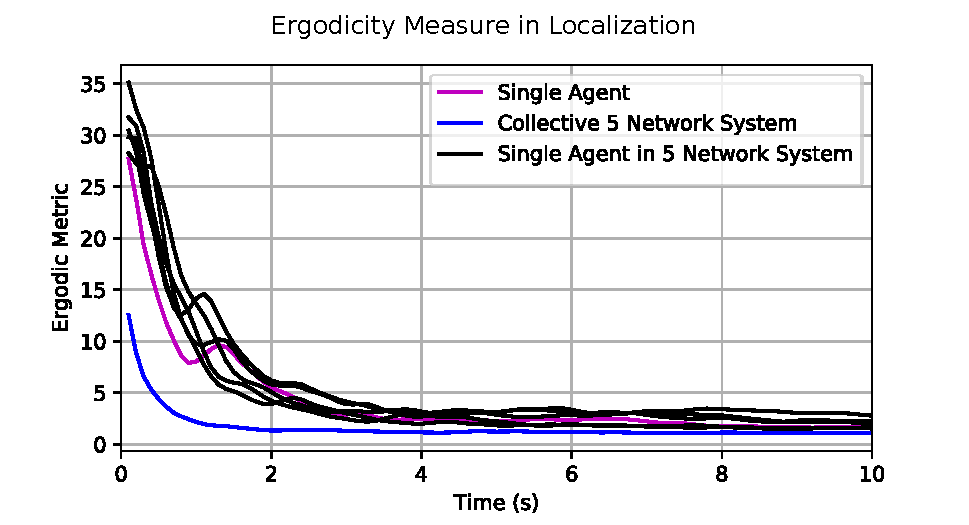
\includegraphics[scale=0.5]{figures/localization_convergence.pdf}
\caption{ Ergodicity measures for a single agent localizing 5 targets versus a 5 agent network localizing 5 targets. Each individual agent's ergodic measure is shown for the 5 agent network. Compared with the single agent, most robots individually have similar ergodic measures. As a connected network utilizing consensus, the ergodic measure is shown to be significantly less. This is due to shared information between agents on where each agent has been, thus each agent explores in a manner that is best for the collective group. }
\label{fig:disloc_conv}
\end{figure}

\subsection{Estimation}


Results for the problem of estimation is presented for a network of 5 autonomous aircraft that is tasked to estimate the terrain of a square grid. The motion of each agent is subject to the dynamics given by
\begin{equation*}
\begin{bmatrix}
\dot{x}  \\
\dot{y} \\
\dot{z} \\
\dot{\theta} \\
\dot{\psi}
\end{bmatrix} =
\begin{bmatrix}
u \cos(\theta) \cos(\psi) \\
u \cos(\theta) \sin(\psi) \\
u \sin(\theta) \\
v \\
w
\end{bmatrix}
\end{equation*}
where $(u,v,w)$ are the control inputs and $u > 0$ such that the aircraft must always be in motion. Each individual agent then takes measurements of the terrain height with which they are currently above\footnote{Each agent has an additional penalty to maintain a specific height above the terrain which prevents collision of the terrain.}. A distributed Kalman filter is used to estimate the terrain height based on the assumption that the terrain can be described as a network of radial-basis functions (RBFs) \cite{du2014radial}. RBFs are typically used to described a continuous surface using a discrete set of radial-basis functions. In this application, the RBFs are used as an estimator which can be used to generate an expected information density. As each agent acquires data, the distributed Kalman filter updates the terrain estimate and then forms a consensus on the estimate based on the network of the agents. The distributed ergodic control then synthesizes control actions that reduce the ergodic metric with respect to the expected information density.

\begin{figure*}[!th]
\centering
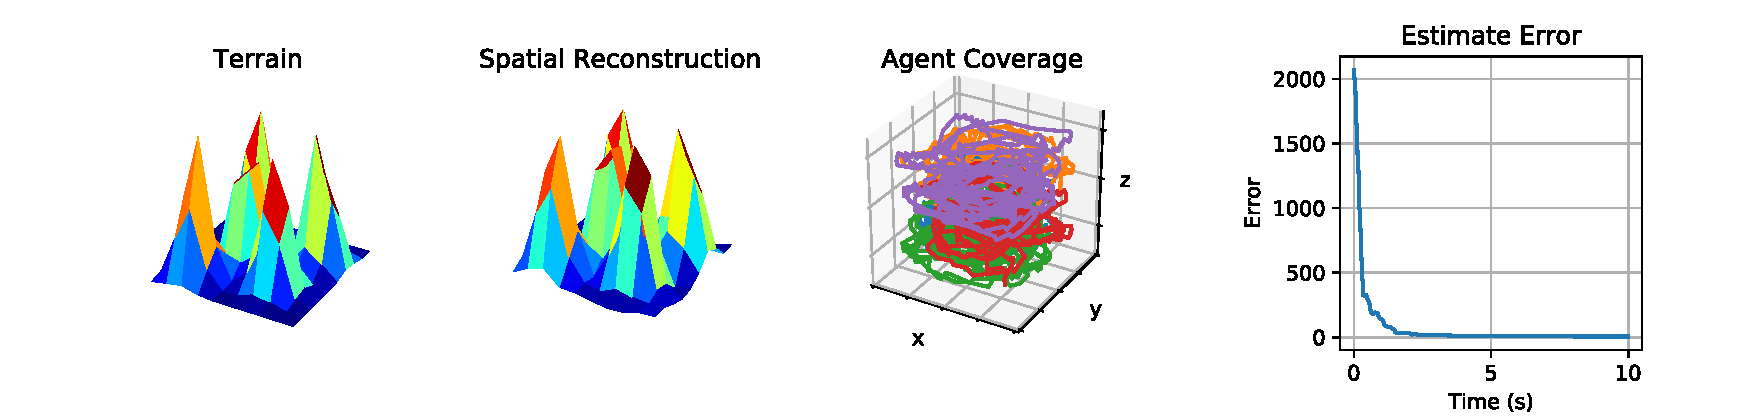
\includegraphics[scale=0.6]{figures/terrain_estimation.pdf}
\caption{ Terrain estimation is shown with a 5 agent aircraft network connected as shown in Fig.~\ref{fig:path}. Aircrafts take height measurements at each sampling rate and reconstruct the terrain based on a a radial-basis-function network. Agent coverage is shown to span the whole space. Estimate error is shown to provide a numerical measure of the accuracy of the spatial reconstruction.  }
\label{fig:estimation}
\end{figure*}

The ground truth terrain is shown in Fig.~\ref{fig:estimation} as well as the estimate for the 5 agent network after 10 second simulation time. For the alloted time, the estimate is shown to converge closely to the ground truth terrain. Although the graph connectivity is not that of a complete graph (a ring graph is used Fig.~\ref{fig:path}), the agent's coverage is still shown to grasp a significant amount of the allotted space for which the aircraft is allowed to travel.

\section{Conclusion} \label{sec:conc}

In this work, ergodic control is formulated as a means to synthesize actions that exhibit exploratory coverage behavior subject to a target statistical distribution. The formulation is then extended into a centralized distributed control problem for active exploration. Using graph theory and distributed optimization, ergodic control is reformulated in a completely distributed manner where information about past exploration is shared amongst agents. The sharing of past exploration provides a consensus on what has been explored and the sensitivity to the next action for each individual agent that reduces the ergodic metric. Various examples that utilize variants of ergodic control problem formulation are used to show improved convergence with additional agents, faster localization time and coverage, and rapid estimation of terrain.

In future work, we will examine the effects of the consensus matrix on the distributed ergodic control and augmentations to the controller to maintain network connectivity for time-varying graph topology.

\bibliographystyle{IEEEtran/IEEEtran}
\bibliography{CDC2017}
\balance

\end{document}
